\chapter{Hluboké Q-učení}

\section{Základní princip}
\subsection{Neuronová síť}

\subsection{Q-učení}
\subsection{Hluboké q-učení}

\section{Využití}
Kde se používá v praxi.


\section{Aplikace}
\subsection{Úvod}
Herní prostředí nám v každém kroku vrací odměnu, kterou oba z hráčů za jejich akci obdrželi. Tuto informaci jsme v experimentech provedených v rámci genetického programování, nevyužili, ale zde budou hrát velkou roli.
Za každý krok, kdy hra ještě neskončila získávají agenti automaticky odměnu 1. Na konci hry agent obdrží vysokou odměnu v případě výhry a v případě prohry naopak získá penalizaci v podobě odměnu vysoké záporné hodnoty. Tyto hodnoty se pro jednotlivé experimenty mírně liší.
Odměnu za výhru, nebo prohru získá agent až na úplném konci hry, to může ztěžovat učící proces. Proto prostředí dává agentům i průběžné menší odměny, pro lepší možnost učení se.

Konkrétně to jsou následující odměny:
\begin{itemize}
    \item Sestřelení asteroidu
        \newline
        Za každý sestřelený asteroid získává agent odměnu hodnoty 5.
    \item Zasažení asteroidem nepřátelské vesmírné lodi
        \newline
        Zranění nepřítele je právě to, co agent potřebuje pro přiblížění se vítězství, proto za každé takové zasažení získává od prostředí odměnu v hodnotě 20.
    \item Zasažení asteroidem vlastní vesmírné lodi
        \newline
        Takový stav je pro agenta znevýhodňující a cílem je se mu vyvarovat, proto za takovýto stav agent od prostředí dostává penalizaci v hodnotě -10.
\end{itemize}


\todo{presunout do kapitoly o deep q}
V rámci učení agentů budeme využívat epsilon-hladového (ang. epsilon-greedy) přístupu. V každém kroku q-učení volíme další akci a epsilon-hladový přístup nám v tom pomáhá následovně.
Vygenerujeme náhodnou hodnotou z intervalu $(0,1)$ a pokud je tato hodnota menší než hodnota epsilon, tak provedeme volbu akce náhodně, v opačném případě volíme nejlepší akce dle q-sítě.
Hodnota epsilon se na počátku inicializuje na hodnotu 1 a po každé zahrané hře se sníží vynásobením koeficientem menším než 1. 
Epsilon-hladový přístup způsobuje, že z počátku učení se zkoušejí náhodné akce a v průběhu přechází ze zkoušení nových akcí do prohledávání již osvědčených akcí.

\todo{presunout do kapitoly o deep q}
\par
V Hlubokém učení se chceme při trénování vyvarovat závislostí na předchozích stavech. K tomu využijeme konceptu přehrávání zkušeností (ang. Experience replay).
Při hraní hry si v každém kroku ukládáme do paměti pětici současného stavu, provedené akce, obdržené odměny, stavu, do kterého jsme se dostali a informace zda hra neskončila.
Po konci zahrání hry následně náhodně vybíráme tyto pětice z paměti a trénování provádíme na nich.






\subsection{Experiment 4: Soupeření s obranným agentem}
V 1. experimentu jsme za pomocí genetického programování hledali agenta, který je úspěšný v souboji s obranným jedincem a využívali jsme k tomu fitness funkci pro určení jak agent v souboji obstál.
Zde, pomocí hlubokého q učení, budeme také učit agenta vzájemnými souboji s obranným agentem, ale budeme namísto fitness funkce používat pro trénování odměny.

S 1. experimentem zde bude také stejný přístup ke vstupům a výstupům. 
Na vstupu budou opět délky všech čtyř akčních plánů a počet kroků před srážkou vesmírné lodi s asteroidem.
A na výstupu čtyři hodnoty reprezentující výběr konkrétního akčního plánu.

Q učení spočívá v učení rozhodování se o akcích. Akce zde v tomto pojetí však nebudou elementární akce, nýbrž akční plány. 
Q-síť bude tedy volit akční plány a proto zde budeme muset provádět mezikrok pro přechod od akčních plánů k akcím.
Vždy nejprve zvolíme akční plán a následně pro pokračování v simulaci hry z vybraného akčního plánu zvolíme první akci.
V tomto experimentu budeme využívat přehrávání zkušeností, tj. budeme průběžně ukládat informace o přechodech do dalších stavů. 
I Zde, pro zapamatování si zkušenosti, platí, že akcí budeme chápat akční plán.


Parametry experimentu:
\begin{itemize}
    \item Na konci hry agent obdrží agent odměnu v hodnotě 2000 v případě výhry a -1000 v případě prohry.
    \item Q-síť je hustá neuronová síť s pěti vstupy, čtyřmi výstupy a jednou skrytou vrstvou. 
    \item Během učení bude zahráno 1500 her.
    \item Konstanta pro snižování epsilon je nastavena na 0.998. To znamená, že například po zahrání 1400 her se bude v další hře volit akce náhodně jen v 6\% případů. 
\end{itemize}

\par
V souboji s obranným agentem se výslednému agentovi podařilo zvítězil pouze ve čtyřech hrách. 
Nepodařilo se nám tedy sice nalézt agenta, který by porážel obranného agenta, ale dosáhli jsme jiného zajímavého výsledku.
Velkým přínosem tohoto experimentu je pestrá strategie nalezeného agenta. Výlsedný agent ve velkém zastoupení používá všechny akční plány (viz \ref{Výsledek experimentu 04}). 
Získali jsme tak agenta, který se brání nejen sestřelováním nepřátelských asteroidů, ale i vyhýbáním se. A díky tomu se agent také pohybuje a nezůstává staticky stát na stejném místě po celou dobu hry.
Toho se nám také podařilo dosáhnout ve 3. experimentu, ale srovnání s agentem získaným ze 3. experimentu je tento agent daleko více obranyschopný.




\begin{figure}[p]\centering
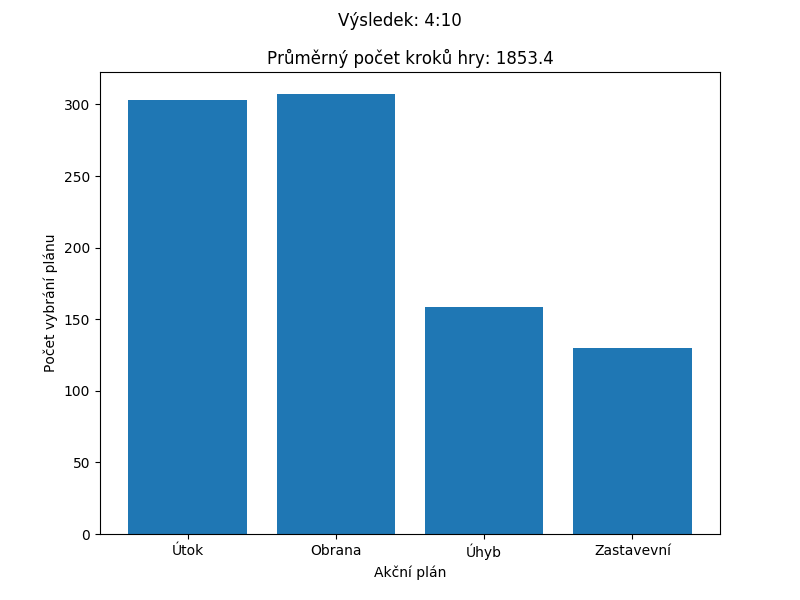
\includegraphics[width=145mm, height=110mm]{./Obrazky/Experiment04Results.png}
\caption{Výsledek experimentu 4}
\label{Výsledek experimentu 04}
\end{figure}

\subsection{Experiment 5: Soupeření s obranným agentem - Rozšířeno}
V předchozím experimentu jsme dosáhli zajímavého chování agenta, ale nepodařilo se nám vyhrávat nad obranným agentem.
Zkusíme proto předchozí experiment rozšířit. 
V tomto experimentu zkusíme rozšířit vstupní argumenty o další, které by mohli agentovi pomoct v rozhodování.

Přidané parametry:
\begin{itemize}
    \item Dvojice počtu zbývajících životů obou agentů            
    \item Počet nebezepčných asteroidů v blízké vzdálenosti od agenta
    \item Celkový současný počet nebezpečných asteroidů v celé hře
\end{itemize}
Snaha všech přidaných argumentů je rozšířit agentovi poznání o současném stavu hry a díky tomu dát agentovi možnost se komplexněji rozhodovat pro akční plány.

Parametry experimentu:
\begin{itemize}
    \item Odměny za finální stav hry zůstávají stejné. Na konci hry agent obdrží agent odměnu v hodnotě 2000 v případě výhry a -1000 v případě prohry.
    \item Q-síť je stejná síť jako v předchozím případě, jen namísto pěti vstupních argumentů, bude nyní přijímat vstupů devět.
    \item V tomto experimentu zkusíme kvůli rozšíření vstupních argumentů také prodloužit trénování sítě, proto bude v rámci trénování zahráno 3000 her.
    \item Adekvátně ke zvýšení počtu zahraných her také zvětšíme konstantu pro snižování epsilon z hodnoty 0.998 na 0.9989. Díky tomu bude stejné pravděpodobnosti 6\% pro volbu náhodné akce dosaženo přibližně po zahrání 2550 her.
\end{itemize}


\todo{obrázek s průběžnými výhrami}\newline
\todo{graf s akčními plány}\newline
\todo{Dokončit 7.Experiment}\newline
\todo{Kapitola o Deep q}\newline
\todo{Transponovat kapitoly o algoritmech a experimentech}\newline
\todo{Naprogramovat spouštění experimentů}\newline
\todo{Popsat spouštění agentů}\newline






\subsection{Experiment 6: Elementární agent proti obrannému agentovi}
V tomto experimentu zkusíme sestoupit od abstrakcí v podobě akčních plánů k elementárním akcím a informacím o stavu.
I zde bude naším cílem trénování zadané neuronové sítě.
Tentokrát nebudeme neuronovou síť používat k volbě akčního plánu, ale přímo k volbě elementární akce.
Výsledný agent rozhodující se pomocí této neuronové sítě bude volit vždy jen jednu akci, proto nebudeme moci využít koncept přepočítávání akčních plánů a agent se bude rozhodovat v každém kroku.

\par
K pěti elementárním akcím přidáme navíc také možnost prázdné akce. Celkem tedy šest možností, proto naše neuronová síť bude mít právě šest výstupů.
Nebudeme volit akční plány, proto nemá ani dobrý smysl používat jejich délky jako vstupy, proto zde můžeme zvolit zcela jiný přístup.
Samotné simulace pro výpočet akčních plánů jsou výpočetně velmi náročné, tedy díky tomu, že zde zvolíme jednodušší přístup, tak budeme schopni, oproti předchozímu experimentu, zahrát v rámci trénování větší množství her.

\par
Vstupy neuronové sítě jsem si zvolil následující hodnoty:
\begin{itemize}
    \item Vektor pohybu vesmírné lodi
    \item Úhel natočení vesmírné lodi
    \item Počet uplynulých kroků od posledního výstřelu
    \item Relativní poloha nepřátelské lodi
    \item Relativní polohy tří nejbližších nebezpečných asteroidů
\end{itemize}

Jako nepřátelského agenta v tomto experimentu jsem zvolil agenta obranného.
Epsilon bylo nastaveno na 0.9985. Pro trénování bylo zahráno 10000 her.



% 10000_base_action_DQ_stable_deffensive_opponent_added_dense_layer_model_1
% 10000_base_action_DQ_stable_deffensive_opponent_added_dense_layer_1.txt

Výsledný agent proti obrannému agentovi nedopadl úspěšně. V souboji byl jednoznačně poražen se skóre 0:10.
V přehledu používaných akcí během souboje vidíme, že elementární agent používal v drtivé většině rotaci a střely.
To v praxi znamená, že se agent naučil točit dokola a kdykoliv může, tak vystřelit. Tato strategie skutečně přináší nějaké výsledky.
Agent tak rozstřeluje kolem letící asteroidy do všech různých směrů, avšak rozhoduje se pro toto chování bezmyšlenkovitě. Nemíří na žádné konkrétní asteroidy, ani na nepřátelskou loď.
Největší slabinou je, že agent se prakticky vůbec nenaučil bránit se. Zřejmě bylo v rámci trénování neuronové sítě nalezeno lokální optimum.

\begin{figure}[p]\centering
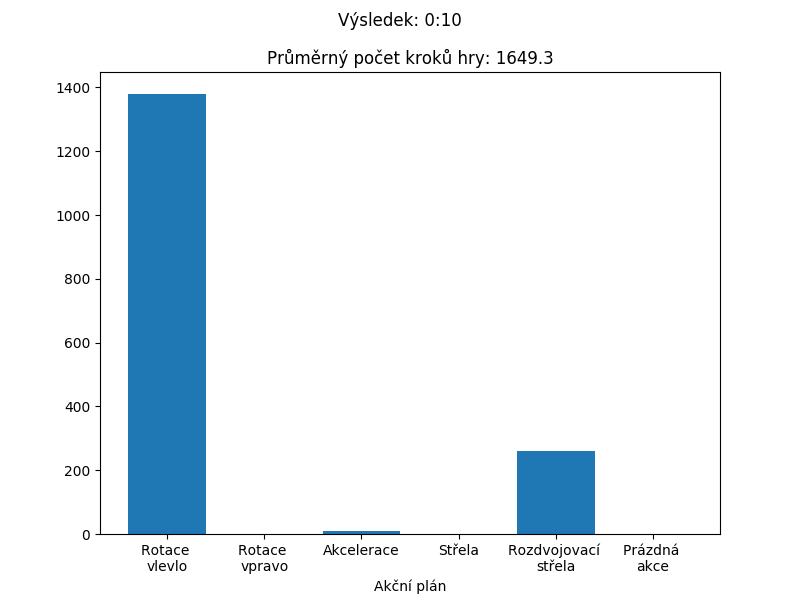
\includegraphics[width=145mm, height=110mm]{./Obrazky/Experiment05Results.png}
\caption{Výsledek experimentu 6}
\label{Výsledek experimentu 06}
\end{figure}
    



\subsection{Experiment 7: Dva elementární agenti}
Tento experiment rozšiřuje experiment předchozí. Budeme opět pracovat s elementárním agentem reprezentovaného neuronovou sítí stejného formátu jako v předhozím případě.
Tentokrát ale ale nebudeme v trénování hrát hry proti obrannému agentovi, nýbrž proti dalšímu elementárnímu agentovi, který bude také zároveň trénován.
Budeme tedy trénovat dvě neuronové sítě najednou. Teoreticky bychom měli dosáhnout vzájemného adaptivního učení, kde se každý z agentů snaží zlepšovat proti svému nepříteli a postupně se tak budou oba zlepšovat.
\par
Parametry trénování: ... 




,